\documentclass[12pt,a4paper]{ctexart}

\usepackage[UTF8]{ctex}
\usepackage{geometry}
\usepackage{graphicx}
\usepackage{xcolor}
\usepackage{tikz}
\usepackage{fontspec}
\usepackage{setspace}
\usepackage{enumitem}
\usepackage{booktabs}
\usepackage{array}
\usepackage{longtable}
\usepackage{hyperref}
\usepackage{fancyhdr}
\usepackage{titlesec}
\usepackage{multicol}
\usepackage{xurl}
\usepackage{tocloft}

\renewcommand{\cfttoctitlefont}{\hfill\bfseries\Large}
\renewcommand{\cftaftertoctitle}{\hfill}
\geometry{left=2.5cm,right=2.5cm,top=2.5cm,bottom=2.5cm}

\definecolor{black}{RGB}{0,0,0}
\definecolor{mainblue}{RGB}{0,82,147}
\definecolor{accentgold}{RGB}{180,140,60}
\definecolor{lightgray}{RGB}{245,245,245}
\definecolor{darkgray}{RGB}{80,80,80}
\definecolor{mainred}{RGB}{230,1,45}

\hypersetup{
    colorlinks=true,
    linkcolor=black,
    urlcolor=mainblue,
    citecolor=mainblue,
    pdfborder={0 0 0}
}

\pagestyle{fancy}
\fancyhf{}
\fancyhead[L]{\small\color{darkgray}\textbf{量子行业每周新闻洞察}}
\fancyhead[R]{\small\color{darkgray}\textbf{总第{{ issue_no }}期}}
\fancyfoot[C]{\thepage}
\renewcommand{\headrulewidth}{0.4pt}
\renewcommand{\footrulewidth}{0pt}

\titleformat{\section}
    {\Large\bfseries\color{mainred}}
    {\thesection、}{0em}{}
\titleformat{\subsection}
    {\large\bfseries\color{mainred}}
    {\thesubsection、}{0em}{}

\newcolumntype{L}[1]{>{\raggedright\arraybackslash}p{#1}}
\newcolumntype{C}[1]{>{\centering\arraybackslash}p{#1}}

\begin{document}

% ==================== 封面 ====================
\begin{titlepage}
\begin{tikzpicture}[remember picture,overlay]
    \fill[mainred] ([yshift=-0.5cm]current page.north west) rectangle ([yshift=-1.2cm]current page.north east);
    \fill[mainred] ([yshift=1.2cm]current page.south west) rectangle ([yshift=0.5cm]current page.south east);
\end{tikzpicture}

\vspace*{4cm}

\begin{center}
    {\fontsize{44}{52}\selectfont\bfseries\color{black} \textbf{量子行业每周新闻洞察}}

    \vspace{0.8cm}

    {\fontsize{16}{22}\selectfont\color{darkgray} {{ start_date }} — {{ end_date }} }
    {\fontsize{16}{22}\selectfont\color{darkgray} \textbf{WEEKLY NEWS}}

    \vspace{1.5cm}

    {\fontsize{20}{26}\selectfont\color{mainred}\textbf{（总第\textbf{ {{ issue_no }} }期）}}

    \vspace{4cm}

    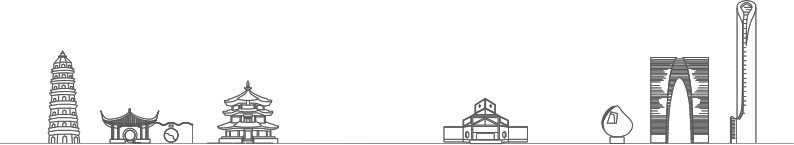
\includegraphics[width=\textwidth]{Cover_Suzhou.png}

    \vfill

    {\fontsize{12}{16}\selectfont\color{darkgray} 量子科技长三角产业创新中心\\编制：战略情报与成果专利室、产业发展部（理事会办公室）}
\end{center}
\end{titlepage}

% ==================== 目录 ====================
\pagenumbering{roman}
\newpage
\tableofcontents

\newpage

% ==================== 摘要 ====================
\pagenumbering{arabic}
\setcounter{page}{1}
\section*{摘要}
\addcontentsline{toc}{section}{摘要}

\textbf{宏观态势：}

{{ summaries['宏观态势'] }}

\textbf{科技前沿：}

{{ summaries['科技前沿'] }}

\textbf{产品动态：}

{{ summaries['产品动态'] }}

\textbf{企业资讯：}

{{ summaries['企业资讯'] }}

\textbf{资本运作：}

{{ summaries['资本运作'] }}

{% if conferences %}
% ==================== 会议列表 ====================
{
    \newpage
    \section*{ {{ conf_month }}月量子科技行业国内、国际会议}
    \addcontentsline{toc}{section}{ {{ conf_month }}月量子科技行业国内、国际会议}
    \scriptsize
    \begin{longtable}{C{0.8cm}L{2.5cm}L{3cm}L{7cm}}
        \toprule[1.5pt]
        \textbf{序号} & \textbf{日期} & \textbf{地点} & \textbf{会议名称} \\
        \midrule
        \endfirsthead
        \toprule
        \textbf{序号} & \textbf{日期} & \textbf{地点} & \textbf{会议名称} \\
        \midrule
        \endhead
        \bottomrule
        \endfoot
        {% for conf in conferences %}
        {{ loop.index }} & {{ conf.date_str }} & {{ conf.location }} & {{ conf.name }} \\
        \midrule[0.05pt]
        {% endfor %}
    \end{longtable}
}
{% endif %}

{% if tenders %}
% ==================== 招投标列表 ====================
{
    \newpage
    \section*{本周新增预采招标线索追踪}
    \addcontentsline{toc}{section}{本周预采招标线索追踪}
    \scriptsize
    \begin{longtable}{C{0.6cm}L{1.8cm}L{1.8cm}L{2.4cm}C{1.2cm}C{1.5cm}C{1.5cm}L{1.5cm}}
        \toprule[1.5pt]
        \textbf{序号} & \textbf{项目名称} & \textbf{项目基本情况} & \textbf{项目主体单位} & \textbf{项目规模（万元）} & \textbf{发布时间} & \textbf{预采时间} &  \textbf{信息来源}  \\
        \midrule
        \endfirsthead
        \toprule
        \textbf{序号} & \textbf{项目名称} & \textbf{项目基本情况} & \textbf{项目主体单位} & \textbf{项目规模（万元）} & \textbf{发布时间} & \textbf{预采时间} & \textbf{信息来源}   \\
        \midrule
        \endhead
        \bottomrule
        \endfoot
        {% for t in tenders %}
        {{ loop.index }} & {{ t.name }} & {{ t.desc }} & {{ t.unit }} & {{ t.scale }} & {{ t.pub_date }} & {{ t.pre_date }} & {% if t.url %}\href{ {{ t.url }} }{点击此处}{% else %}{% endif %} \\
        \midrule[0.05pt]
        {% endfor %}
    \end{longtable}
}
{% endif %}

{% if patents %}
% ==================== 专利动态 ====================
\newpage
\section{专利动态}
\vspace{-0.5em}
\noindent\rule{\linewidth}{1.5pt}
{% for group in patents %}
\subsection{ {{ group.category }} }
{% for p in group.items %}
\subsubsection{ {{ p.title }} }
申请人：{{ p.applicant }}
发明人：{{ p.inventor }}
公开日/授权日：{{ p.date }}

摘要：

{{ p.abstract }}

\noindent\textbf{专利链接：}\url{ {{ p.url }} }
{% endfor %}
{% endfor %}
{% endif %}

% ==================== 宏观态势 ====================
\newpage
\section{宏观态势}
\vspace{-0.5em}
\noindent\rule{\linewidth}{1.5pt}
{% for art in categories['宏观态势'] %}
\subsection{ {{ art.title }} }

{{ art.content }}

\noindent\textbf{报道链接：}\url{ {{ art.liangke_url }} }
{% endfor %}

% ==================== 科技前沿 ====================
\newpage
\section{科技前沿}
\vspace{-0.5em}
\noindent\rule{\linewidth}{1.5pt}
{% for art in categories['科技前沿'] %}
\subsection{ {{ art.title }} }

{{ art.content }}

\noindent\textbf{报道链接：}\url{ {{ art.liangke_url }} }
{% endfor %}

% ==================== 产品动态 ====================
\newpage
\section{产品动态}
\vspace{-0.5em}
\noindent\rule{\linewidth}{1.5pt}
{% for art in categories['产品动态'] %}
\subsection{ {{ art.title }} }

{{ art.content }}

\noindent\textbf{报道链接：}\url{ {{ art.liangke_url }} }
{% endfor %}

% ==================== 企业资讯 ====================
\newpage
\section{企业资讯}
\vspace{-0.5em}
\noindent\rule{\linewidth}{1.5pt}
{% for art in categories['企业资讯'] %}
\subsection{ {{ art.title }} }

{{ art.content }}

\noindent\textbf{报道链接：}\url{ {{ art.liangke_url }} }
{% endfor %}

% ==================== 资本运作 ====================
\newpage
\section{资本运作}
\vspace{-0.5em}
\noindent\rule{\linewidth}{1.5pt}
{% for art in categories['资本运作'] %}
\subsection{ {{ art.title }} }

{{ art.content }}

\noindent\textbf{报道链接：}\url{ {{ art.liangke_url }} }
{% endfor %}

\end{document}
